\chapter{Results}

\label{ch:Results}


%
%
%
%
%
\section{Learning Generative Factors in Dense Latent Spaces}

\begin{itemize}
\item Reconstruction 
\item Sampling
\item MNIST, Frey, Pong, Space Invaders and Breakout
\item We wish to be able to achieve a similar result with altering activations of specific filters
\end{itemize}


%
%
%
%
%
\section{Single Latent Filter}

\begin{itemize}
\item Consider two architectures: shallow and deep
\item Consider Pong, Space Invaders (in progress) and Breakout
\item Plot reconstruction loss and KL divergence
\item Show reconstructions and convolutional layers of each
\item Show mean activations of filters
\item Alter latent space variable and show reconstruction
\end{itemize}

\begin{figure*}[h!]
\centering
\captionsetup{justification=centering}
\begin{multicols}{4}
    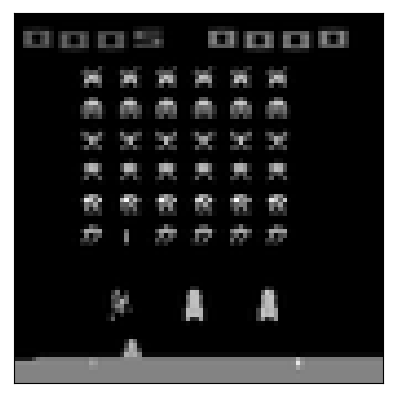
\includegraphics[scale=0.4]{figures/results/latent_image/beta_1_sample_0_original.png}
    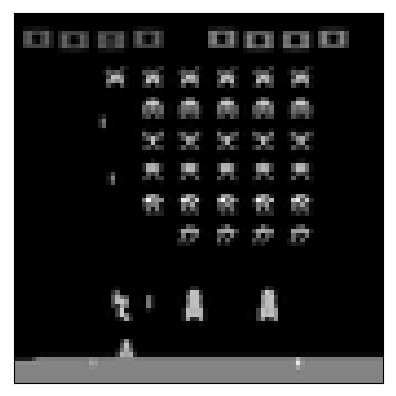
\includegraphics[scale=0.4]{figures/results/latent_image/beta_1_sample_1_original.png}
    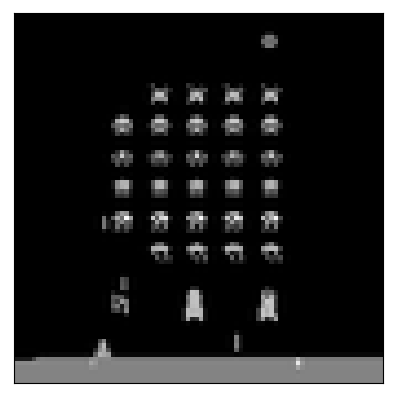
\includegraphics[scale=0.4]{figures/results/latent_image/beta_1_sample_2_original.png}
    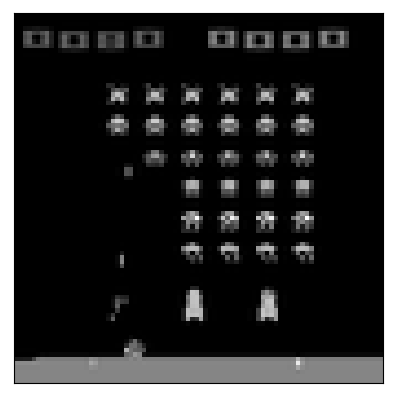
\includegraphics[scale=0.4]{figures/results/latent_image/beta_1_sample_3_original.png}
\end{multicols}
\begin{multicols}{4}
    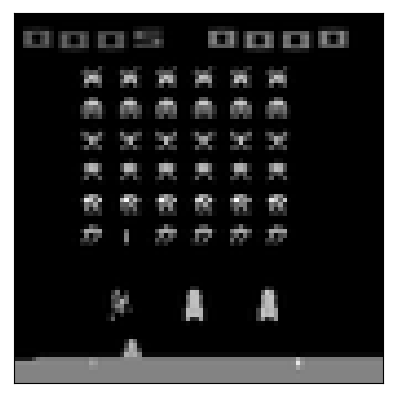
\includegraphics[scale=0.4]{figures/results/latent_image/beta_1_sample_0_reconstructed.png}
    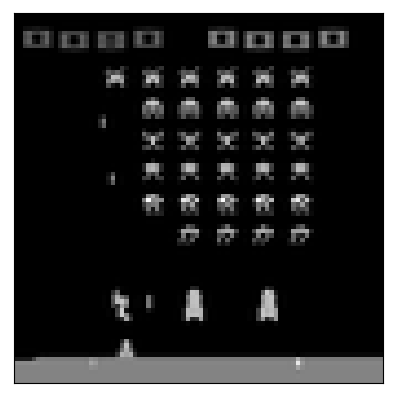
\includegraphics[scale=0.4]{figures/results/latent_image/beta_1_sample_1_reconstructed.png}
    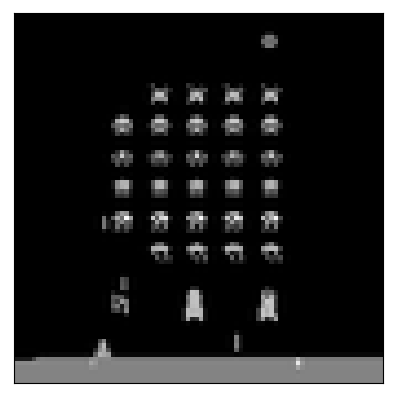
\includegraphics[scale=0.4]{figures/results/latent_image/beta_1_sample_2_reconstructed.png}
    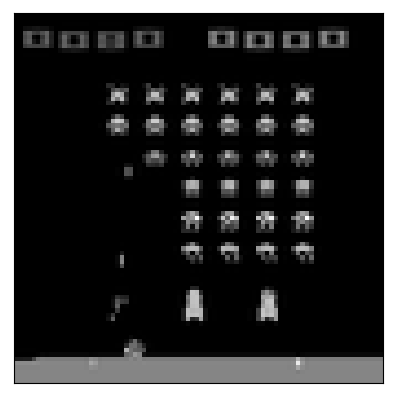
\includegraphics[scale=0.4]{figures/results/latent_image/beta_1_sample_3_reconstructed.png}
\end{multicols}
\caption{\textbf{Top row:} Original frames from Space Invaders. \textbf{Bottom row:} Corresponding reconstructions.}
\label{fig:latent_image_originals_and_reconstructions}
\end{figure*}


\begin{figure*}[h!]
\centering
\captionsetup{justification=centering}
\begin{multicols}{4}
    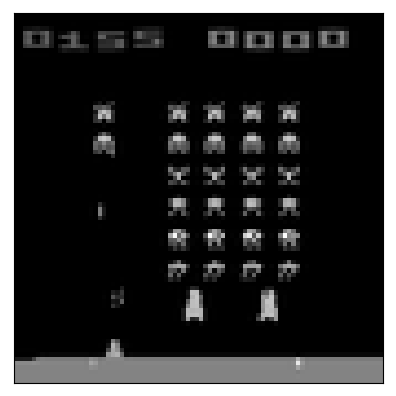
\includegraphics[scale=0.4]{figures/results/latent_image/beta_1_sample_10_original.png}
    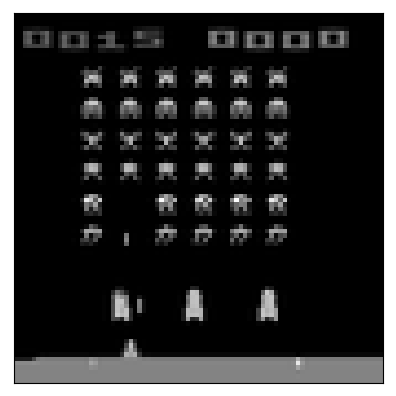
\includegraphics[scale=0.4]{figures/results/latent_image/beta_1_sample_30_original.png}
    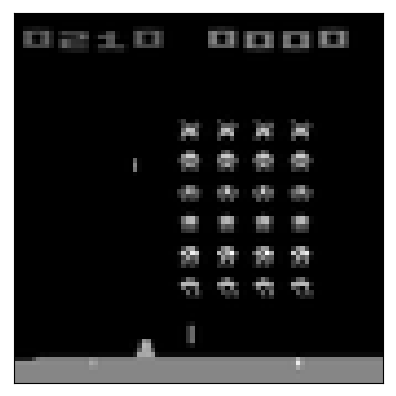
\includegraphics[scale=0.4]{figures/results/latent_image/beta_1_sample_70_original.png}
    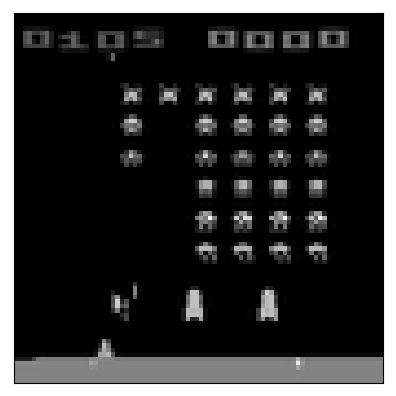
\includegraphics[scale=0.4]{figures/results/latent_image/beta_1_sample_90_original.png}
\end{multicols}
\begin{multicols}{4}
    
\includegraphics[scale=0.3]{figures/results/latent_image/beta_1_sample_10_latent.png}
    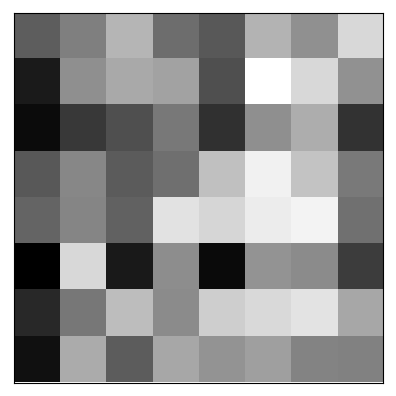
\includegraphics[scale=0.3]{figures/results/latent_image/beta_1_sample_30_latent.png}
    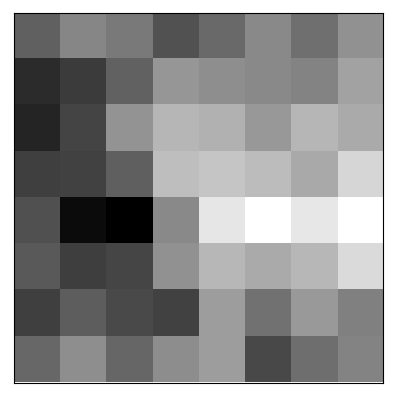
\includegraphics[scale=0.3]{figures/results/latent_image/beta_1_sample_70_latent.png}
    
\includegraphics[scale=0.3]{figures/results/latent_image/beta_1_sample_90_latent.png}
\end{multicols}
\caption{\textbf{Top row:} Original frames from Space Invaders. \textbf{Bottom row:} Corresponding latent images.}
\label{fig:latent_image_originals_and_latent_spaces}
\end{figure*}


\begin{figure*}[h!]
\centering
\captionsetup{justification=centering}
\begin{multicols}{4}
    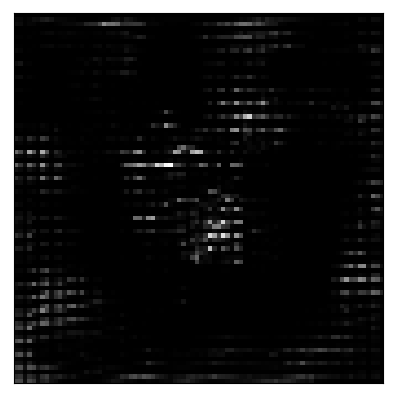
\includegraphics[scale=0.4]{figures/results/latent_image/beta_1_prior_sample_0.png}
    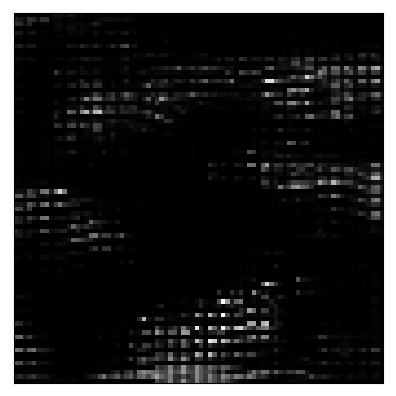
\includegraphics[scale=0.4]{figures/results/latent_image/beta_1_prior_sample_1.png}
    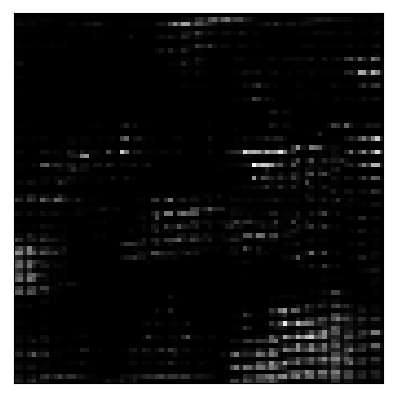
\includegraphics[scale=0.4]{figures/results/latent_image/beta_1_prior_sample_2.png}
    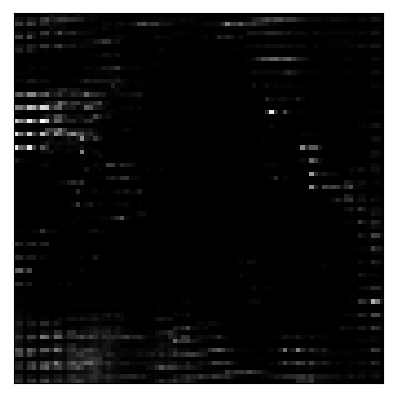
\includegraphics[scale=0.4]{figures/results/latent_image/beta_1_prior_sample_3.png}
\end{multicols}
\caption{Samples from prior.}
\label{fig:latent_image_originals_prior_samples}
\end{figure*}


\begin{figure*}[h!]
\centering
\captionsetup{justification=centering}
\begin{multicols}{4}
    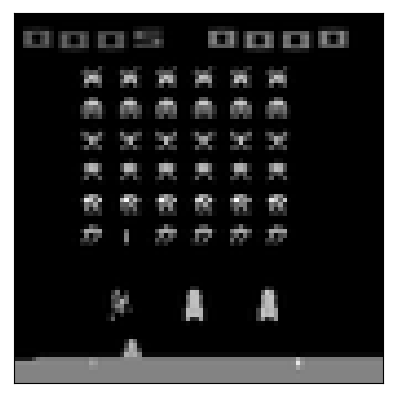
\includegraphics[scale=0.4]{figures/results/latent_image/beta_1_posterior_sample_original.png}
    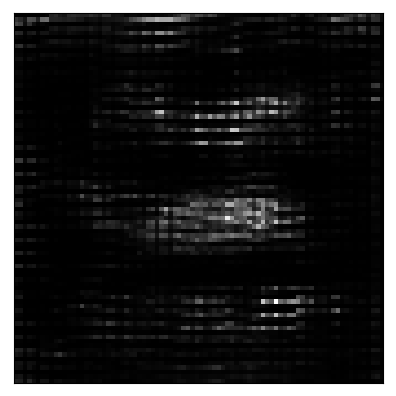
\includegraphics[scale=0.4]{figures/results/latent_image/beta_1_posterior_sample_0.png}
    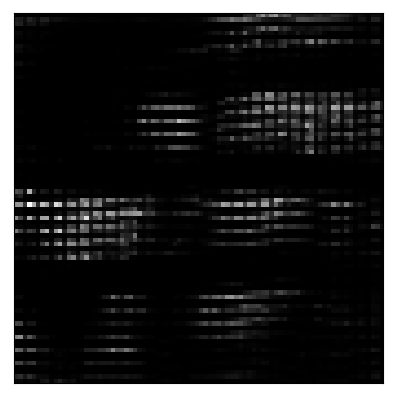
\includegraphics[scale=0.4]{figures/results/latent_image/beta_1_posterior_sample_5.png}
    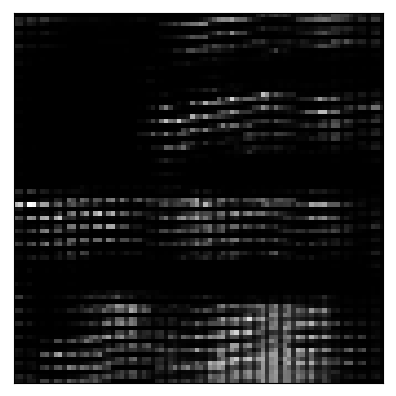
\includegraphics[scale=0.4]{figures/results/latent_image/beta_1_posterior_sample_10.png}
\end{multicols}
\caption{Samples from posterior.}
\label{fig:latent_image_originals_posterior_samples}
\end{figure*}


%
%
%
%
%
\section{Disentangling Latent Neurons}
\begin{itemize}
\item Consider two architectures: shallow and deep
\item Consider Pong, Space Invaders (in progress) and Breakout
\item Plot reconstruction loss and KL divergence
\item Show reconstructions and convolutional layers of each
\item Show mean activations of filters
\item Alter latent space variable and show reconstruction
\item Add noise to filters
\end{itemize}


%
%
%
%
%
\section{Disentangling Latent Filters Using Averages}
\begin{itemize}
\item Consider two architectures: shallow and deep
\item Consider Pong, Space Invaders (done) and Breakout
\item Plot reconstruction loss and KL divergence
\item Show reconstructions and convolutional layers of each
\item Show mean activations of filters
\item Alter latent space variable and show reconstruction
\item Add noise to filters
\end{itemize}


%
%
%
%
%
\section{Decoupling Latent Filters Using Weighted-Averages}
\begin{itemize}
\item Consider two architectures: shallow and deep
\item Consider Pong, Space Invaders (done) and Breakout
\item Plot reconstruction loss and KL divergence
\item Show reconstructions and convolutional layers of each
\item Show mean activations of filters
\item Alter latent space variable and show reconstruction
\item Add noise to filters
\end{itemize}


%
%
%
%
%
\section{Separating Colour Spaces}
\begin{itemize}
\item Consider two architectures: shallow and deep
\item Consider Pong, Space Invaders (in progress) and Breakout
\item Plot reconstruction loss and KL divergence
\item Show reconstructions and convolutional layers of each
\item Show mean activations of filters
\item Alter latent space variable and show reconstruction
\item Add noise to filters
\end{itemize}


%
%
%
%
%
\section{Orthogonal Convolutions}
\begin{itemize}
\item Consider two architectures: shallow and deep
\item Consider Pong, Space Invaders and Breakout
\item Plot reconstruction loss and KL divergence
\item Show reconstructions and convolutional layers of each
\item Alter latent space variable and show reconstruction
\item Add noise to filters
\end{itemize}


%
%
%
%
%
\section{Winner Takes All}
\begin{itemize}
\item Consider two architectures: shallow and deep
\item Consider Pong, Space Invaders and Breakout
\item Plot reconstruction loss and KL divergence
\item Show reconstructions and convolutional layers of each
\item Show mean activations of filters
\item Alter latent space variable and show reconstruction
\item Show samples from prior and posterior
\item Add noise to filters
\end{itemize}


%
%
%
%
%
\section{The No Free Lunch Relationship Between Reconstruction Loss and KL Divergence}

\begin{itemize}
\item Vary $\beta$ and plot BCE and KL
\item Show example images for different $\beta$
\item Consider Space Invaders, Pong and Breakout
\end{itemize}

%
%
%
%
%
\section{Using Batch Normalisation With Convolutional Variational Latent Spaces}

\begin{itemize}
\item Consider single architecture 
\item Batch norm before, after, both, and none
\end{itemize}